\documentclass[10pt]{article}\usepackage[]{graphicx}\usepackage[]{color}
%% maxwidth is the original width if it is less than linewidth
%% otherwise use linewidth (to make sure the graphics do not exceed the margin)
\makeatletter
\def\maxwidth{ %
  \ifdim\Gin@nat@width>\linewidth
    \linewidth
  \else
    \Gin@nat@width
  \fi
}
\makeatother

\definecolor{fgcolor}{rgb}{0.345, 0.345, 0.345}
\newcommand{\hlnum}[1]{\textcolor[rgb]{0.686,0.059,0.569}{#1}}%
\newcommand{\hlstr}[1]{\textcolor[rgb]{0.192,0.494,0.8}{#1}}%
\newcommand{\hlcom}[1]{\textcolor[rgb]{0.678,0.584,0.686}{\textit{#1}}}%
\newcommand{\hlopt}[1]{\textcolor[rgb]{0,0,0}{#1}}%
\newcommand{\hlstd}[1]{\textcolor[rgb]{0.345,0.345,0.345}{#1}}%
\newcommand{\hlkwa}[1]{\textcolor[rgb]{0.161,0.373,0.58}{\textbf{#1}}}%
\newcommand{\hlkwb}[1]{\textcolor[rgb]{0.69,0.353,0.396}{#1}}%
\newcommand{\hlkwc}[1]{\textcolor[rgb]{0.333,0.667,0.333}{#1}}%
\newcommand{\hlkwd}[1]{\textcolor[rgb]{0.737,0.353,0.396}{\textbf{#1}}}%
\let\hlipl\hlkwb

\usepackage{framed}
\makeatletter
\newenvironment{kframe}{%
 \def\at@end@of@kframe{}%
 \ifinner\ifhmode%
  \def\at@end@of@kframe{\end{minipage}}%
  \begin{minipage}{\columnwidth}%
 \fi\fi%
 \def\FrameCommand##1{\hskip\@totalleftmargin \hskip-\fboxsep
 \colorbox{shadecolor}{##1}\hskip-\fboxsep
     % There is no \\@totalrightmargin, so:
     \hskip-\linewidth \hskip-\@totalleftmargin \hskip\columnwidth}%
 \MakeFramed {\advance\hsize-\width
   \@totalleftmargin\z@ \linewidth\hsize
   \@setminipage}}%
 {\par\unskip\endMakeFramed%
 \at@end@of@kframe}
\makeatother

\definecolor{shadecolor}{rgb}{.97, .97, .97}
\definecolor{messagecolor}{rgb}{0, 0, 0}
\definecolor{warningcolor}{rgb}{1, 0, 1}
\definecolor{errorcolor}{rgb}{1, 0, 0}
\newenvironment{knitrout}{}{} % an empty environment to be redefined in TeX

\usepackage{alltt}

\usepackage{amsmath,amssymb,amsthm}
\usepackage{fancyhdr,url,hyperref}
\usepackage{graphicx,xspace}
\usepackage{subfigure}
\usepackage{tikz}
\usetikzlibrary{arrows,decorations.pathmorphing,backgrounds,positioning,fit,through}

\oddsidemargin 0in  %0.5in
\topmargin     0in
\leftmargin    0in
\rightmargin   0in
\textheight    9in
\textwidth     6in %6in
%\headheight    0in
%\headsep       0in
%\footskip      0.5in

\newtheorem{thm}{Theorem}
\newtheorem{cor}[thm]{Corollary}
\newtheorem{obs}{Observation}
\newtheorem{lemma}{Lemma}
\newtheorem{claim}{Claim}
\newtheorem{definition}{Definition}
\newtheorem{question}{Question}
\newtheorem{answer}{Answer}
\newtheorem{problem}{Problem}
\newtheorem{solution}{Solution}
\newtheorem{conjecture}{Conjecture}

\pagestyle{fancy}

\lhead{\textsc{Prof. McNamara}}
\chead{\textsc{SDS/MTH 220: Lecture notes}}
\lfoot{}
\cfoot{}
%\cfoot{\thepage}
\rfoot{}
\renewcommand{\headrulewidth}{0.2pt}
\renewcommand{\footrulewidth}{0.0pt}

\newcommand{\ans}{\vspace{0.25in}}
\newcommand{\R}{{\sf R}\xspace}
\newcommand{\cmd}[1]{\texttt{#1}}

\rhead{\textsc{September 13, 2017}}
\IfFileExists{upquote.sty}{\usepackage{upquote}}{}
\begin{document}

\paragraph{Agenda}
\begin{enumerate}
  \itemsep0em
  \item Experimental Design
\end{enumerate}


\paragraph{Stratified sampling simulation}

  Recall the stratifield sampling exercise from last time, and suppose that hourly wages were normally distributed with means \$25, \$15, \$22, and \$15, among the 90 women working full-time, 18 women working part-time, 9 men working full-time, and 63 men working part-time, respectively. The following \R code builds a data frame that represents one possible reality. 

\begin{knitrout}
\definecolor{shadecolor}{rgb}{0.969, 0.969, 0.969}\color{fgcolor}\begin{kframe}
\begin{alltt}
\hlstd{staff} \hlkwb{=} \hlkwd{c}\hlstd{(}\hlkwd{rep}\hlstd{(}\hlstr{"women-ft"}\hlstd{,} \hlnum{90}\hlstd{),} \hlkwd{rep}\hlstd{(}\hlstr{"women-pt"}\hlstd{,} \hlnum{18}\hlstd{),} \hlkwd{rep}\hlstd{(}\hlstr{"men-ft"}\hlstd{,} \hlnum{9}\hlstd{),} \hlkwd{rep}\hlstd{(}\hlstr{"men-pt"}\hlstd{,} \hlnum{63}\hlstd{))}
\hlstd{wage} \hlkwb{=} \hlkwd{c}\hlstd{(}\hlkwd{rnorm}\hlstd{(}\hlnum{90}\hlstd{,} \hlkwc{mean} \hlstd{=} \hlnum{25}\hlstd{),} \hlkwd{rnorm}\hlstd{(}\hlnum{18}\hlstd{,} \hlnum{15}\hlstd{),} \hlkwd{rnorm}\hlstd{(}\hlnum{9}\hlstd{,} \hlnum{22}\hlstd{),} \hlkwd{rnorm}\hlstd{(}\hlnum{63}\hlstd{,} \hlnum{15}\hlstd{))}
\hlstd{ds} \hlkwb{=} \hlkwd{data.frame}\hlstd{(staff, wage)}
\hlkwd{head}\hlstd{(ds)}
\end{alltt}
\begin{verbatim}
##      staff     wage
## 1 women-ft 24.24287
## 2 women-ft 25.49924
## 3 women-ft 25.73812
## 4 women-ft 25.80283
## 5 women-ft 26.09438
## 6 women-ft 26.54672
\end{verbatim}
\begin{alltt}
\hlkwd{nrow}\hlstd{(ds)}
\end{alltt}
\begin{verbatim}
## [1] 180
\end{verbatim}
\end{kframe}
\end{knitrout}

Note that wages are similar \emph{within} the four groups, but dissimilar \emph{among} the groups. This command will draw separate densities for the four groups on the same plot. 

\begin{knitrout}
\definecolor{shadecolor}{rgb}{0.969, 0.969, 0.969}\color{fgcolor}\begin{kframe}
\begin{alltt}
\hlkwd{require}\hlstd{(mosaic)}
\end{alltt}


{\ttfamily\noindent\color{warningcolor}{\#\# Warning: package 'dplyr' was built under R version 3.4.1}}\begin{alltt}
\hlkwd{qplot}\hlstd{(}\hlkwc{x} \hlstd{= wage,} \hlkwc{color} \hlstd{= staff,} \hlkwc{geom} \hlstd{=} \hlstr{"density"}\hlstd{,} \hlkwc{data} \hlstd{= ds)}
\end{alltt}
\end{kframe}

{\centering 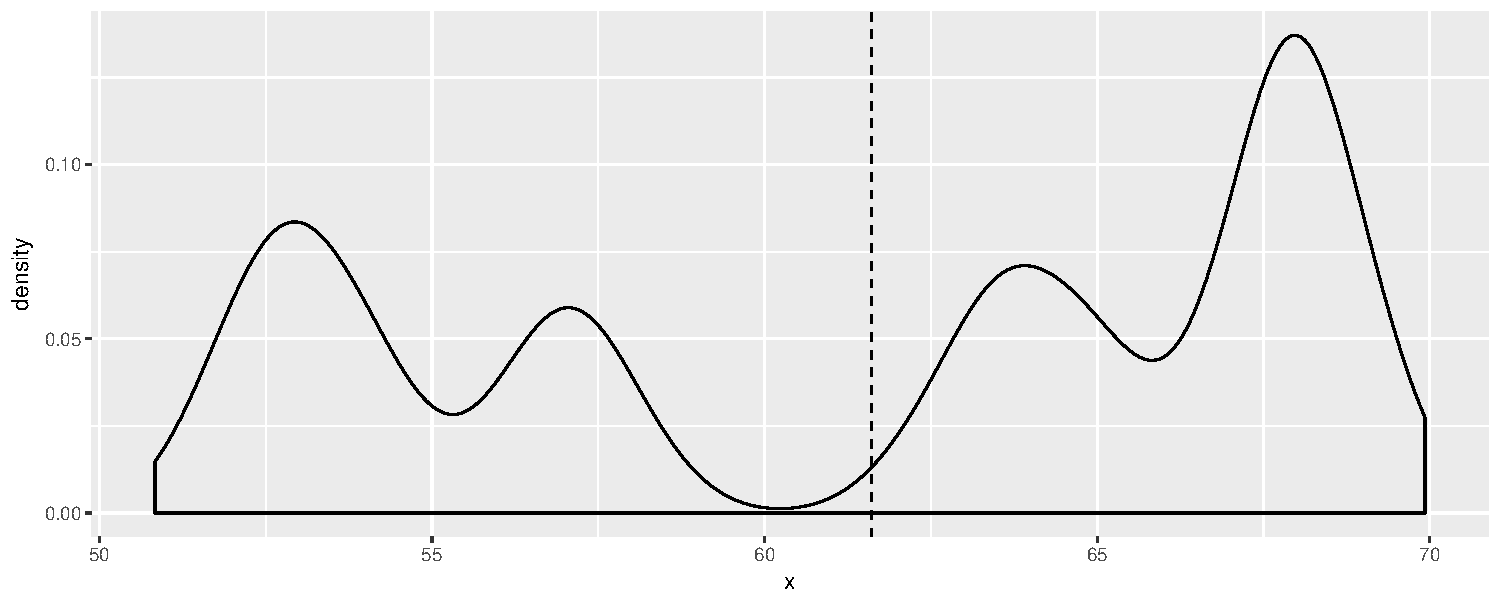
\includegraphics[width=\maxwidth]{figure/unnamed-chunk-2-1} 

}



\end{knitrout}

We want to estimate the mean wage among all 180 workers. In this case, since we know the wage of all of the workers, we can just compute it. 
  
\begin{knitrout}
\definecolor{shadecolor}{rgb}{0.969, 0.969, 0.969}\color{fgcolor}\begin{kframe}
\begin{alltt}
\hlkwd{mean}\hlstd{(}\hlopt{~}\hlstd{wage,} \hlkwc{data} \hlstd{= ds)}
\end{alltt}
\begin{verbatim}
## [1] 20.36328
\end{verbatim}
\end{kframe}
\end{knitrout}
  
But recall that for the purposes of this exercise, we don't actually know all 180 wages, and we are asked to sample 40 of them. We can take a \emph{simple random sample} and compute the mean wage within that sample.

\begin{knitrout}
\definecolor{shadecolor}{rgb}{0.969, 0.969, 0.969}\color{fgcolor}\begin{kframe}
\begin{alltt}
\hlcom{# simple random sampling}
\hlkwd{mean}\hlstd{(}\hlopt{~}\hlstd{wage,} \hlkwc{data} \hlstd{=} \hlkwd{sample}\hlstd{(ds,} \hlnum{40}\hlstd{))}
\end{alltt}
\begin{verbatim}
## [1] 20.00752
\end{verbatim}
\end{kframe}
\end{knitrout}

Note that this is close to the actual mean wage, but not the same. Note also that each time we take a different random sample, we get a different mean wage in that sample. 

Now let's implement the \emph{stratified sampling} scheme.

\begin{knitrout}
\definecolor{shadecolor}{rgb}{0.969, 0.969, 0.969}\color{fgcolor}\begin{kframe}
\begin{alltt}
\hlcom{# Stratified sampling}
\hlstd{strat_samp} \hlkwb{<-} \hlkwd{bind_rows}\hlstd{(}
  \hlkwd{sample}\hlstd{(}\hlkwd{filter}\hlstd{(ds, staff} \hlopt{==} \hlstr{"women-ft"}\hlstd{),} \hlnum{20}\hlstd{),}
  \hlkwd{sample}\hlstd{(}\hlkwd{filter}\hlstd{(ds, staff} \hlopt{==} \hlstr{"women-pt"}\hlstd{),} \hlnum{4}\hlstd{),}
  \hlkwd{sample}\hlstd{(}\hlkwd{filter}\hlstd{(ds, staff} \hlopt{==} \hlstr{"men-ft"}\hlstd{),} \hlnum{2}\hlstd{),}
  \hlkwd{sample}\hlstd{(}\hlkwd{filter}\hlstd{(ds, staff} \hlopt{==} \hlstr{"men-pt"}\hlstd{),} \hlnum{14}\hlstd{)}
\hlstd{)}
\hlkwd{mean}\hlstd{(}\hlopt{~}\hlstd{wage,} \hlkwc{data} \hlstd{= strat_samp)}
\end{alltt}
\begin{verbatim}
## [1] 20.3993
\end{verbatim}
\end{kframe}
\end{knitrout}

Again, the stratified sample mean is close to the actual value, but not the same. It will also differ each time we take a different random sample. So why might we prefer stratified sampling over simple random sampling?
  
Let's compare the \emph{distribution} of sample means if we do this many, many times!

\begin{knitrout}
\definecolor{shadecolor}{rgb}{0.969, 0.969, 0.969}\color{fgcolor}\begin{kframe}
\begin{alltt}
\hlcom{# Comparison}
\hlstd{SRS} \hlkwb{=} \hlkwd{do}\hlstd{(}\hlnum{1000}\hlstd{)} \hlopt{*} \hlkwd{mean}\hlstd{(}\hlopt{~}\hlstd{wage,} \hlkwc{data} \hlstd{=} \hlkwd{sample}\hlstd{(ds,} \hlnum{40}\hlstd{))}
\hlstd{STR} \hlkwb{=} \hlkwd{do}\hlstd{(}\hlnum{1000}\hlstd{)} \hlopt{*} \hlkwd{mean}\hlstd{(}\hlopt{~}\hlstd{wage,} \hlkwc{data} \hlstd{=} \hlkwd{bind_rows}\hlstd{(}
                                \hlkwd{sample}\hlstd{(}\hlkwd{filter}\hlstd{(ds, staff} \hlopt{==} \hlstr{"women-ft"}\hlstd{),} \hlnum{20}\hlstd{),}
                                \hlkwd{sample}\hlstd{(}\hlkwd{filter}\hlstd{(ds, staff} \hlopt{==} \hlstr{"women-pt"}\hlstd{),} \hlnum{4}\hlstd{),}
                                \hlkwd{sample}\hlstd{(}\hlkwd{filter}\hlstd{(ds, staff} \hlopt{==} \hlstr{"men-ft"}\hlstd{),} \hlnum{2}\hlstd{),}
                                \hlkwd{sample}\hlstd{(}\hlkwd{filter}\hlstd{(ds, staff} \hlopt{==} \hlstr{"men-pt"}\hlstd{),} \hlnum{14}\hlstd{)}
\hlstd{))}
\hlstd{sim} \hlkwb{=} \hlkwd{bind_rows}\hlstd{(SRS, STR)} \hlopt
  \hlkwd{mutate}\hlstd{(}\hlkwc{scheme} \hlstd{=} \hlkwd{rep}\hlstd{(}\hlkwd{c}\hlstd{(}\hlstr{"simple"}\hlstd{,} \hlstr{"statified"}\hlstd{),} \hlkwc{each} \hlstd{=} \hlnum{1000}\hlstd{))}
\hlkwd{qplot}\hlstd{(}\hlkwc{data} \hlstd{= sim,} \hlkwc{x} \hlstd{= mean,} \hlkwc{color} \hlstd{= scheme,} \hlkwc{geom} \hlstd{=} \hlstr{"density"}\hlstd{)}
\end{alltt}
\end{kframe}

{\centering 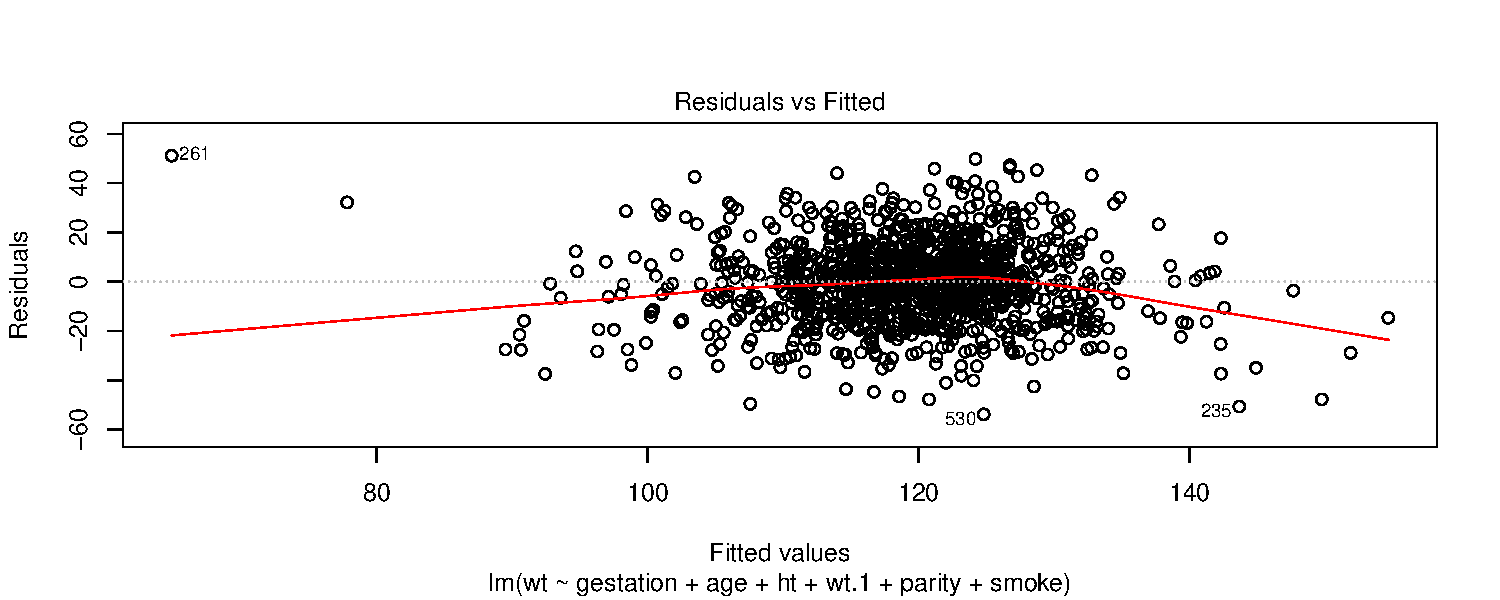
\includegraphics[width=\maxwidth]{figure/unnamed-chunk-6-1} 

}



\end{knitrout}


\paragraph{Experimental Design}

% Provide a definition and an example for where each of these sampling terms might be used
% \begin{enumerate}
% \itemsep0.28in
%   \item blocks of experimental units
%   \item double-blind
% %  \item random assignment
% %  \item random selection
%   \item confounding
% %  \item multistage sampling
% %  \item stratified random sample
% %  \item sampling distribution
%   \item bias
%   \item informed consent
%   \item nonresponse
% \end{enumerate}

\begin{enumerate}
%  \itemsep2in
%\item 3.116 (page 234) \textsc{Prostate treatment study using Canada's national health records}: A large observational study used records from Canada's national health care system to compare the effectiveness of two ways to treat prostate disease. The two treatments are traditional surgery and a new method that does not require surgery. The records described many patients whose doctors had chosen one or the other method. The study found that patients treated by the new method were significantly more likely to die within 8 years. 
%  \begin{enumerate}
%    \item Further study of the data showed that this conclusion was wrong. The extra deaths among patients who received the new treatment could be explained by lurking variables. What lurking variables might be confounded with a doctor's choice of surgical or nonsurgical treatment?
%    \item You have 300 prostate patients who are willing to serve as subjects in an experiment to compare the two methods. Use a diagram to outline the design of a randomized comparative experiment. 
%  \end{enumerate}
  % MMC, 7e, 3.108 (page 223)
  \item What is the best way to answer each of the questions below: an experiment, a sample survey, or an observational study that is not a sample survey? Explain your choices.
  \begin{enumerate}
    \itemsep0.25in
    \item Are people generally satisfied with how things are going in the country right now?
    \item Do college students learn basic accounting better in a classroom or using an online course?
    \item How long do your teachers wait on average after they ask their class a question?
    \ans
  \end{enumerate}
  
  % MMC, 7e, 2.140 (page 153)
  \item A study showed that women who work in the production of computer chips have abnormally high numbers of miscarriages. The union claimed that exposure to chemicals used in production caused the miscarriages. Another possible explanation is that these workers spend most of their work time standing up. Illustrate these relationships in a diagram.
  
  \vspace{2in}
  
  \item A study shows that there is a positive correlation between the size of a hospital (measured by its number of beds $x$) and the median number of days $y$ that patients remain in the hospital. Does this mean that you can shorten a hospital stay by choosing a small hospital? Use a diagram to explain the association.
  
  \vspace{2in}
  
%  \item 3.124 (page 235) \textsc{Compare two doses of a drug}: A drug manufacturer is studying how a new drug behaves in patients. Investigators compare two doses: 5 mg and 10 mg. The drug can be administered by injection, by a skin patch, or by intravenous drip. Concentration in the blood after 30 minutes (the response variable) may depend on both the does and on the method of administration.
%  \begin{enumerate}
%    \item Make a sketch that describes the treatments formed by combining dosage and method. Then use a diagram to outline a completely randomized design for this two-factor experiment. 
%    \item ``How many subjects?" is a tough issue. We will explain the basic ideas in Ch. 6. What can you say now about the advantage of using larger groups of subjects?
%  \end{enumerate}
  % MMC, 7e, 3.137 (page 226)
  \item Students sign up to be subjects in a psychology experiment. When they arrive, they are told that interviews are running late and are taken to a waiting room. The experimenters then stage a theft of a valuable object left in the waiting room. Some subjects are alone with the thief, and others are in pairs -- these are the treatments being compared. Will the subject report the theft? The students had agreed to take part in an unspecified study, and the true nature of the experiment is explained to them afterward. Do you think this study is ethically OK?
  \ans
\end{enumerate}


\paragraph{Activity}

For each of the following pairs of variables, a statistically signficant positive relationship has been observed. Identify a potential lurking variable that might cause the spurious correlation.
\begin{enumerate}
  \itemsep0.5in
  \item The amount of ice cream sold in New England and the number of deaths by drowning
  \item The salary of U.S. ministers and the price of vodka
  \item The number of doctors in a region and the number of crimes committed in that region
  \item The number of storks sighted and the population of Oldenburg, Germany, over a six-year period
  \item The amount of coffee consumed and the prevalence of lung cancer
\end{enumerate}

% 
% \newpage
% 
% \subsection*{Instructor's Notes}
% 
% \begin{itemize}
%   \item Confounding: when a variable is correlated with both the response and explanatory variable. Confounding may lead to spurious relationships.
%   \item Common response: When a lurking variable causes change in both the response and explanatory variables
%   \item Causality: correlation does not imply causation! Be especially wary of time as a confounder. Consider the relationship between the number of Big Macs eaten and the number of people who have walked on the moon. Causality cannot be inferred from observational data -- only from randomized, controlled experiments.
%   \item Four Principles of Experimental Design (1.5.1, pg. 17):
%   \begin{enumerate}
%     \item Controlling: evening out differences (e.g. using a control group to simulate the action of the treatment group)
%     \item Randomization: randomly assign patients to groups, etc.
%     \item Replication: a study performed multiple times should get the same results!
%     \begin{enumerate}
%       \item replication: different people get the same results with different data
%       \item reproducibility: different people get the same results with the same data
%     \end{enumerate}
%     Reproducibility is huge issue! \href{http://www.nature.com/nature/focus/reproducibility/index.html}{Nature editorial series}
%     \item Blocking: dividing groups proactively to compare like with like
%   \end{enumerate}
%   \item Blinding and double-blinding: prevent bias on the part of researchers and patients
% \end{itemize}
% 
% \begin{figure}
%   \centering
%   \subfigure[Causation]{
%   \begin{tikzpicture}[auto,node distance=2cm,thick
%     ,var/.style={circle,draw}
%     ,causation/.style={->, thick}
%     ,association/.style={<->, dashed}]
%   %
%   \node[var] (x) {$x$};
%   \node[var] (y) [right of=x] {$y$};
%   %
%   \draw[causation] (x) to (y);
%   \draw[association, bend left] (x) to (y);
%   \end{tikzpicture}
%   }
%   \hspace{1in}
%   \subfigure[Common Response]{
%   \begin{tikzpicture}[auto,node distance=2cm,thick
%     ,var/.style={circle,draw}
%     ,causation/.style={->, thick}
%     ,association/.style={<->, dashed}]
%   %
%   \node[var] (x) {$x$};
%   \node[var] (y) [right of=x] {$y$};
%   \node[var] (z) [below of=x] {$z$};
%   %
%   \draw[causation] (z) to (x);
%   \draw[causation] (z) to (y);
%   \draw[association, bend left] (x) to (y);
%   \end{tikzpicture}
%   }
%   \hspace{1in}
%   \subfigure[Confounding]{
%   \begin{tikzpicture}[auto,node distance=2cm,thick
%     ,var/.style={circle,draw}
%     ,causation/.style={->, thick}
%     ,association/.style={<->, dashed}]
%   %
%   \node[var] (x) {$x$};
%   \node[var] (y) [right of=x] {$y$};
%   \node[var] (z) [below of=x] {$z$};
%   %
%   \draw[causation] (x) to (y);
%   \draw[causation] (z) to (y);
%   \draw[association, bend left] (x) to (y);
%   \draw[association, bend left] (z) to (x);
%   \draw[association, bend right] (z) to (y);
%   \end{tikzpicture}
%   }
% \end{figure}


\end{document}
